% !TeX spellcheck = id_ID
\documentclass[a4paper,12pt]{article}
\usepackage[bahasa]{babel}
\usepackage{graphicx}
\usepackage{multirow}
\usepackage{enumitem}
\usepackage{listings}
\graphicspath{ {./img/} }
\begin{document}
\title{TRANSFORMASI ERD KE DALAM RELASIONAL TABEL}
%\author{Aldzikri Dwijayanto Prathama \\ {\small 195410189}}
\author{Aldzikri Dwijayanto Prathama
	\\195410189}
\makeatletter
\begin{titlepage}
	\begin{center}
        {\LARGE \bfseries \@title }\\[14ex]
		
\includegraphics[scale=.8]{logo}\\[4ex]
		{\large \@author}\\[20ex]
		{\large \bfseries {SEKOLAH TINGGI MANAJEMEN INFORMATIKA DAN KOMPUTER
				AKAKOM YOGYAKARTA}}
	\end{center}


%{\large \@date} 
\end{titlepage}
\makeatother
%\maketitle

\section*{\centering{ERD DATA PENJUALAN BARANG ELEKTRONIK}}
\begin{center}
    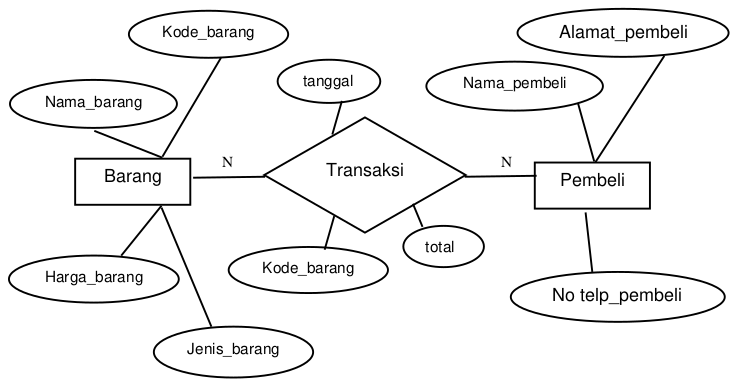
\includegraphics[width=\linewidth]{1.png} 
\end{center}

\section*{Barang}
\begin{table}[h!]
\begin{tabular}{|l|l|l|l|}
\hline
Kode\_barang & Nama\_barang & Harga\_barang & Jenis\_barang \\ \hline
             &              &               &               \\ \hline
\end{tabular}
\end{table}

\section*{Pembeli}
\begin{table}[h!]
\begin{tabular}{|l|l|l|}
\hline
Nama\_pembeli & Alamat\_pembeli & NoTelp\_pembeli \\ \hline
              &                 &                 \\ \hline
\end{tabular}
\end{table}

\section*{Transaksi}
\begin{table}[h!]
\begin{tabular}{|l|l|l|}
\hline
Kode\_barang & Tanggal & Total \\ \hline
             &         &       \\ \hline
\end{tabular}
\end{table}

\end{document}
